%======================================================================
\section{결과}
\label{sec:results}

\begin{yoji}
두 규칙 모두, 수정 분석에서도 등록 분석에서도 만족하지 못했어요. C-PR은 새 허락 쌍에서는 송금 걷기를 크게 앞섰지만, 새 송금자에서는 허용 폭보다 더 뒤졌어요. 트레이더 라벨에서는 수정 분석에서 송금 걷기와 같았지만 구간이 허용 폭 안에 들지 못했고, 등록 분석에서는 송금 걷기보다 못했어요. 라벨을 안 뒤에 계산한 대비에서, 새 허락 쌍은 두 분석 모두 받은 허락 수를 넘는 걷기가 없었어요. 새 송금자는 수정 분석에서만 송금 입차수가 C-PR과 AWP보다 나았고, 등록 분석에서는 AWP가 송금 입차수보다 나았어요.
\end{yoji}

소절마다 먼저 수정 분석, 곧 규칙에 따른 재분석을 보고하고, 이어서 등록 분석, 곧 규칙을 정할 때 시험하려던 분석을 보고해요. 표~\ref{tab:holdout}와~\ref{tab:contrasts}, 그림~\ref{fig:forest}와~\ref{fig:sweep}이 두 분석을 모두 보여 줘요.

\subsection{같은 기간: 규칙 A의 부 부분은 실패}
\label{sec:res-window}

매칭 코호트에서 $\lambda=0.5$의 C-PR은 모든 가족에서 두 층 사이에 놓여요.
\begin{itemize}
\item \textbf{수정 분석.} 송금 가족에서 0.400 [0.385, 0.416]으로, 송금 걷기의 구간 [0.691, 0.709]보다 한참 아래예요. 허락 가족에서 0.449 [0.437, 0.463]으로, 허락 걷기의 구간 [0.550, 0.572]보다 아래예요. 시빌 안정성 가족에서는 0.142 [0.128, 0.156]으로, 허락 걷기(0.028 [0.014, 0.042])보다 위지만 송금 걷기(0.402 [0.389, 0.417])보다 아래예요.
\item \textbf{등록 분석.} 같은 모양이에요. 0.296 [0.289, 0.303] 대 [0.522, 0.534], 0.418 [0.412, 0.423] 대 [0.506, 0.517], 그리고 0.129 [0.124, 0.134]가 0.020 [0.015, 0.026]과 0.311 [0.304, 0.317] 사이에 있어요.
\end{itemize}
그래서 부 기준의 세 부분은 두 분석 모두에서 실패해요. 짝지은 대비도 같은 말을 해요. 송금 가족에서 C-PR에서 송금 걷기를 뺀 값은 수정 분석에서 −0.300 [−0.318, −0.281], 등록 분석에서 −0.232 [−0.239, −0.224]예요. 허락 가족에서 C-PR에서 허락 걷기를 뺀 값은 −0.112 [−0.124, −0.100]과 −0.094 [−0.099, −0.088]이에요. 이 점검들은 그래프를 만드는 바로 그 사건에서 나와요. 그래서 점수가 어떤 구성개념을 따라가는지 보여 줄 뿐, 바깥의 증거는 아니에요~\cite{cronbach1955construct}.

\begin{puri}[점검 가족은 무엇인가요?]
같은 종류의 사건으로 만든 점검 지표를 묶은 것이에요. 송금 가족은 송금에서, 허락 가족은 허락에서 나와요. 시빌 안정성 가족은 들어오는 상대 가운데 서로 다른 상대의 몫, 활동 기간, 활동한 달 수로 이뤄져요. 이 점검들은 그래프를 만드는 사건에서 나오므로, 점수가 어떤 구성개념을 따라가는지 보여 줄 뿐 바깥의 증거가 아니에요.
\end{puri}

\subsection{W0: 규칙 A의 주 부분은 실패}

표~\ref{tab:holdout}는 모든 점수를 나중 라벨과 견주고, 표~\ref{tab:contrasts}는 대비를, 그림~\ref{fig:forest}는 규칙이 정한 대비를 보여 줘요.
\begin{itemize}
\item \textbf{수정 분석.} A1은 성립해요. 새 허락 쌍에서 C-PR은 허락 걷기보다 나쁘지 않아요(+0.031 [0.021, 0.042]). A2는 실패해요. 새 송금자에서 C-PR은 송금 걷기보다 못해요(−0.030 [−0.040, −0.020]). 주 부분이 실패했으므로, 규칙 A는 “C-PR이 한 층만 걷는 걷기를 이기는가”에 ‘아니요’로 답해요.
\item \textbf{등록 분석.} 규칙 A가 시험하려던 분석이에요. 같은 판정이에요. A1은 +0.008 [0.003, 0.013], A2는 −0.030 [−0.034, −0.026]이에요.
\end{itemize}

\begin{figure}[!ht]
\centering
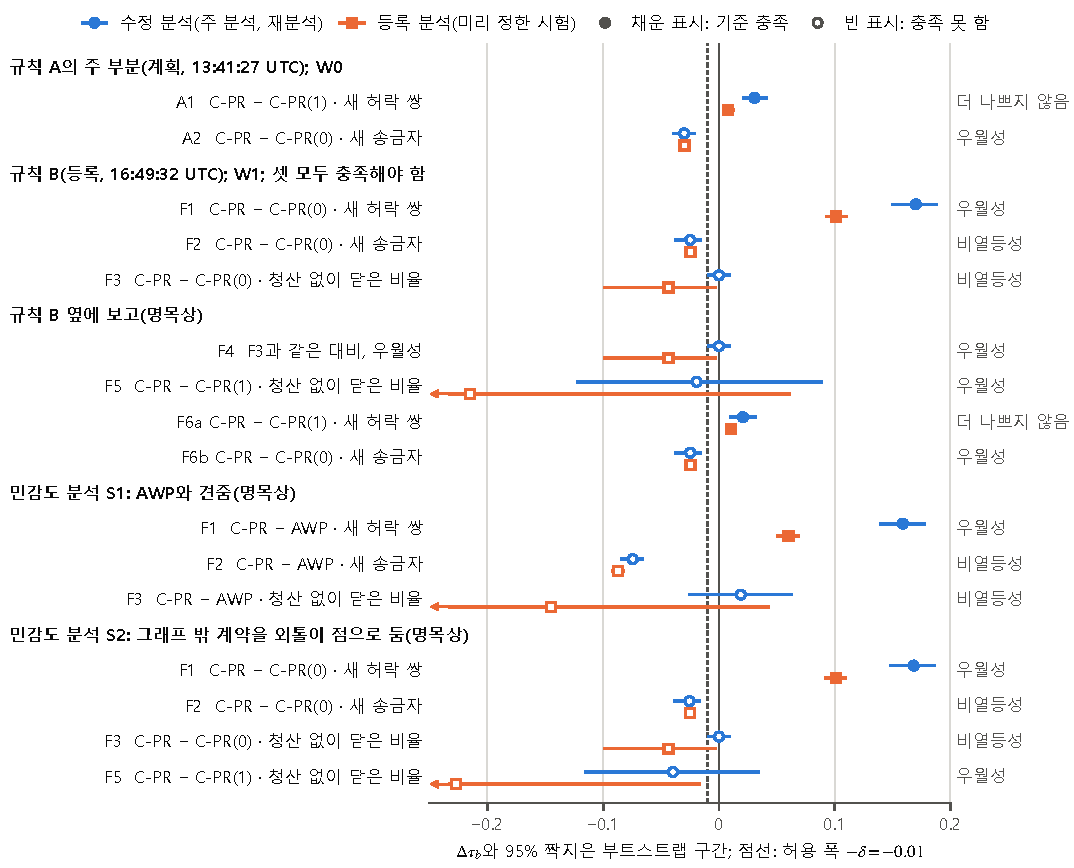
\includegraphics[width=\linewidth]{figures/fig_contrasts.pdf}
\caption{규칙 A와 B가 정한 대비, 규칙 B 옆에 보고하기로 등록한 결과, 그리고 등록한 민감도 분석 두 개. 95\% 짝지은 부트스트랩 구간이에요(다시 뽑기 400번, 시드 42). 동그라미는 수정 분석이에요. 주 분석이고, 달러 금액, 다섯 토큰, 동결 직전 12개월의 점수를 등록 결과를 안 뒤에 정해서 같은 규칙으로 다시 한 재분석이에요. 네모는 등록 분석, 곧 미리 정한 시험이에요. 채운 표시는 기준 충족, 빈 표시는 충족 못 함이에요. 점선은 허용 폭 $-\delta=-0.01$이고, 화살표는 그린 범위를 넘어가는 구간 끝이에요. 규칙을 판정하는 것은 A1--A2와 F1--F3뿐이고, 나머지 판정은 명목상이에요. S1의 F4는 그 F3과 같은 대비라 뺐어요. 값은 표~\ref{tab:contrasts}에 있어요.}
\label{fig:forest}
\end{figure}

\begin{puri}[그림~\ref{fig:forest}를 읽는 법]
한 줄이 대비 하나예요. 점은 $\Delta\tau$, 가로 선은 그 95\% 구간이에요. 세로 실선은 0, 점선은 허용 폭 −0.01이에요. 오른쪽 끝의 글자는 그 줄에 쓰는 기준(우월성, 비열등성, 더 나쁘지 않음)이에요. 예를 들어 F2 줄은 파란 선과 주황 선이 모두 점선의 왼쪽에 통째로 있어요. 두 분석 모두 C-PR이 송금 걷기보다 허용 폭 넘게 뒤졌다는 뜻이에요.
\end{puri}

\begin{table}[!ht]
\centering
\caption{동결 시점의 점수와 나중 라벨 사이의 켄달 $\tau_b$와 95\% 짝지은 부트스트랩 구간}
\label{tab:holdout}
\linespread{1}\selectfont\footnotesize
\setlength{\tabcolsep}{2.4pt}
\begin{tabular}{@{}L{3.5cm}C{2.0cm}C{2.0cm}C{2.0cm}C{2.0cm}C{2.0cm}@{}}
\toprule
\multicolumn{6}{@{}l}{\emph{(가) 수정 분석: 주 분석이며 미리 정한 규칙에 따른 재분석(달러 금액, 다섯 토큰, 12개월 점수 기간)}} \\
 & \multicolumn{2}{c}{W0 스펜더($n=7{,}914$)} & \multicolumn{2}{c}{W1 스펜더($n=7{,}960$)} & W1 트레이더($n=70$) \\
\cmidrule(lr){2-3}\cmidrule(lr){4-5}\cmidrule(l){6-6}
점수 & 새 허락 쌍 & 새 송금자 & 새 허락 쌍 & 새 송금자 & 청산 없이 닫은 비율 \\
\midrule
동결 시점의 받은 허락 수 & \tc{0.392}{[0.377, 0.406]} & \tc{0.284}{[0.267, 0.299]} & \tc{0.381}{[0.365, 0.396]} & \tc{0.269}{[0.250, 0.285]} & \tc{0.394}{[0.261, 0.524]} \\
동결 시점의 송금 입차수 & \tc{0.203}{[0.183, 0.224]} & \tc{0.447}{[0.435, 0.459]} & \tc{0.165}{[0.143, 0.186]} & \tc{0.439}{[0.426, 0.454]} & \tc{0.253}{[0.116, 0.363]} \\
EndorseRank & \tc{0.303}{[0.287, 0.319]} & \tc{0.272}{[0.257, 0.286]} & \tc{0.299}{[0.284, 0.314]} & \tc{0.259}{[0.243, 0.275]} & \tc{0.297}{[0.174, 0.418]} \\
AWP & \tc{0.196}{[0.178, 0.213]} & \tc{0.409}{[0.396, 0.421]} & \tc{0.157}{[0.137, 0.178]} & \tc{0.398}{[0.386, 0.412]} & \tc{0.263}{[0.140, 0.379]} \\
C-PR ($\lambda=1$), 허락 걷기 & \tc{0.298}{[0.282, 0.313]} & \tc{0.267}{[0.250, 0.282]} & \tc{0.295}{[0.280, 0.310]} & \tc{0.257}{[0.241, 0.274]} & \tc{0.302}{[0.177, 0.425]} \\
C-PR ($\lambda=0.75$) & \tc{0.327}{[0.311, 0.342]} & \tc{0.327}{[0.313, 0.339]} & \tc{0.316}{[0.298, 0.330]} & \tc{0.315}{[0.299, 0.329]} & \tc{0.284}{[0.160, 0.398]} \\
C-PR ($\lambda=0.5$), 주 설정 & \tc{0.329}{[0.312, 0.343]} & \tc{0.336}{[0.322, 0.348]} & \tc{0.316}{[0.300, 0.330]} & \tc{0.324}{[0.308, 0.337]} & \tc{0.282}{[0.162, 0.397]} \\
C-PR ($\lambda=0.25$) & \tc{0.329}{[0.312, 0.343]} & \tc{0.345}{[0.330, 0.357]} & \tc{0.315}{[0.299, 0.328]} & \tc{0.332}{[0.317, 0.346]} & \tc{0.282}{[0.162, 0.397]} \\
C-PR ($\lambda=0$), 송금 걷기 & \tc{0.178}{[0.160, 0.197]} & \tc{0.366}{[0.351, 0.378]} & \tc{0.146}{[0.126, 0.168]} & \tc{0.348}{[0.335, 0.363]} & \tc{0.282}{[0.162, 0.394]} \\
S-PR & \tc{0.190}{[0.171, 0.209]} & \tc{0.377}{[0.363, 0.389]} & \tc{0.162}{[0.140, 0.184]} & \tc{0.367}{[0.354, 0.381]} & \tc{0.300}{[0.175, 0.411]} \\
\bottomrule
\end{tabular}
\end{table}

\begin{table}[!ht]
\ContinuedFloat
\centering
\caption{(이어서) 등록 분석}
\linespread{1}\selectfont\footnotesize
\setlength{\tabcolsep}{2.4pt}
\begin{tabular}{@{}L{3.5cm}C{2.0cm}C{2.0cm}C{2.0cm}C{2.0cm}C{2.0cm}@{}}
\toprule
\multicolumn{6}{@{}l}{\emph{(나) 등록 분석: 미리 정한 시험(원래 단위, 모든 ERC-20 토큰)}} \\
 & \multicolumn{2}{c}{W0 스펜더($n=33{,}101$)} & \multicolumn{2}{c}{W1 스펜더($n=34{,}587$)} & W1 트레이더($n=70$) \\
\cmidrule(lr){2-3}\cmidrule(lr){4-5}\cmidrule(l){6-6}
점수 & 새 허락 쌍 & 새 송금자 & 새 허락 쌍 & 새 송금자 & 청산 없이 닫은 비율 \\
\midrule
동결 시점의 받은 허락 수 & \tc{0.252}{[0.244, 0.260]} & \tc{0.156}{[0.148, 0.166]} & \tc{0.262}{[0.255, 0.269]} & \tc{0.179}{[0.171, 0.186]} & \tc{0.394}{[0.261, 0.524]} \\
동결 시점의 송금 입차수 & \tc{0.148}{[0.138, 0.158]} & \tc{0.302}{[0.294, 0.310]} & \tc{0.145}{[0.135, 0.155]} & \tc{0.303}{[0.296, 0.309]} & \tc{0.331}{[0.209, 0.441]} \\
EndorseRank & \tc{0.241}{[0.234, 0.248]} & \tc{0.226}{[0.219, 0.234]} & \tc{0.233}{[0.226, 0.240]} & \tc{0.210}{[0.203, 0.217]} & \tc{0.306}{[0.176, 0.421]} \\
AWP & \tc{0.196}{[0.187, 0.206]} & \tc{0.340}{[0.333, 0.348]} & \tc{0.177}{[0.166, 0.187]} & \tc{0.322}{[0.316, 0.329]} & \tc{0.240}{[0.090, 0.362]} \\
C-PR ($\lambda=1$), 허락 걷기 & \tc{0.228}{[0.219, 0.236]} & \tc{0.122}{[0.113, 0.133]} & \tc{0.227}{[0.219, 0.234]} & \tc{0.133}{[0.125, 0.142]} & \tc{0.310}{[0.181, 0.432]} \\
C-PR ($\lambda=0.75$) & \tc{0.236}{[0.229, 0.243]} & \tc{0.217}{[0.209, 0.226]} & \tc{0.237}{[0.230, 0.244]} & \tc{0.228}{[0.220, 0.236]} & \tc{0.088}{[−0.110, 0.269]} \\
C-PR ($\lambda=0.5$), 주 설정 & \tc{0.236}{[0.229, 0.243]} & \tc{0.224}{[0.216, 0.234]} & \tc{0.237}{[0.230, 0.244]} & \tc{0.235}{[0.227, 0.243]} & \tc{0.095}{[−0.102, 0.274]} \\
C-PR ($\lambda=0.25$) & \tc{0.234}{[0.227, 0.241]} & \tc{0.230}{[0.222, 0.240]} & \tc{0.235}{[0.228, 0.242]} & \tc{0.240}{[0.232, 0.247]} & \tc{0.101}{[−0.096, 0.280]} \\
C-PR ($\lambda=0$), 송금 걷기 & \tc{0.142}{[0.133, 0.151]} & \tc{0.254}{[0.246, 0.262]} & \tc{0.136}{[0.125, 0.145]} & \tc{0.260}{[0.252, 0.266]} & \tc{0.138}{[−0.048, 0.310]} \\
S-PR & \tc{0.177}{[0.167, 0.186]} & \tc{0.245}{[0.236, 0.253]} & \tc{0.169}{[0.159, 0.178]} & \tc{0.251}{[0.244, 0.258]} & \tc{0.312}{[0.183, 0.422]} \\
\bottomrule
\end{tabular}

\vspace{4pt}
\parbox{\linewidth}{\footnotesize W0은 2026년 3월 31일에 점수를 동결하고 2026년 4–6월에 라벨을 세요. W1은 2026년 6월 30일에 동결하고 2026년 7–9월에 세요. 수정 분석은 모든 점수를 그 동결 직전 12개월로, 등록 분석은 2023년 10월 1일부터 추출한 모든 사건으로 만들어요. 스펜더는 동결 시점에 양수의 마지막 허락을 가진 계약이에요. 트레이더는 계약 코드를 가지고, 동결일 그래프의 점이며, 라벨 기간에 포지션을 셋 이상 닫은 GMX V2 계정이에요. 수정 분석에서 W0 스펜더 가운데 1{,}732개가 새 허락 쌍을, 1{,}422개가 새 송금자를 얻었고, W1에서는 1{,}495개와 1{,}371개가 얻었어요. 등록 분석에서는 3{,}403개, 3{,}042개, 2{,}850개, 2{,}812개예요. W1 트레이더 70개 가운데 9개가 청산을 한 번 이상 겪었어요. 받은 허락 수, 송금 입차수, EndorseRank, AWP의 행은 기준 점수이고, 그 비교는 짝 연구~\cite{kwon2026companion}가 모두 보고해요. 구간은 코호트의 계약을 다시 뽑은 짝지은 다시 뽑기 400번(시드 42)에서 왔어요.}
\end{table}

규칙 A에 없던 비교 하나는 반대쪽을 가리켰어요. 규칙 B를 쓸 때 있던 유일한 분석인 등록 분석에서, C-PR은 새 허락 쌍을 송금 걷기 혼자보다 훨씬 잘 줄 세웠어요(0.236 대 0.142, +0.094 [0.085, 0.103]). 이 대비는 라벨을 안 뒤에 살펴본 것이라 가설로 다뤘어요. 그래서 이 연구가 아직 추출하지 않은 창에서 그것을 시험하도록 규칙 B를 썼어요. 수정 점수로는 +0.151 [0.130, 0.170]이에요.

\begin{table}[!p]
\centering
\caption{두 분석의 짝지은 대비: 미리 정한 규칙, 등록한 보고와 민감도 분석, 라벨을 안 뒤에 계산한 대비}
\label{tab:contrasts}
\linespread{1}\selectfont\scriptsize
\setlength{\tabcolsep}{2.2pt}
\begin{tabular}{@{}L{4.45cm}L{1.9cm}C{2.75cm}C{1.45cm}C{2.75cm}C{1.45cm}@{}}
\toprule
 & & \multicolumn{2}{c}{수정 분석(재분석)} & \multicolumn{2}{c}{등록 분석(시험)} \\
\cmidrule(lr){3-4}\cmidrule(l){5-6}
대비($a-b$)와 라벨 & 기준 & $\Delta\tau$ [95\% 구간] & 판정 & $\Delta\tau$ [95\% 구간] & 판정 \\
\midrule
\multicolumn{6}{@{}l}{\emph{규칙 A: 이 연구가 로그를 하나도 추출하기 전에 계획(43d8045)에 정함; W0 스펜더}} \\
A1: C-PR − C-PR ($\lambda=1$), 새 허락 쌍 & 더 나쁘지 않음 & +0.031 [0.021, 0.042] & 성립 & +0.008 [0.003, 0.013] & 성립 \\
A2: C-PR − C-PR ($\lambda=0$), 새 송금자 & 우월성 & −0.030 [−0.040, −0.020] & 실패 & −0.030 [−0.034, −0.026] & 실패 \\
규칙 A의 주 부분(A1과 A2) & & & \textbf{충족 못 함} & & \textbf{충족 못 함} \\
규칙 A의 부 부분(같은 기간) & & & \textbf{충족 못 함} & & \textbf{충족 못 함} \\
\midrule
\multicolumn{6}{@{}l}{\emph{규칙 B: 이 연구가 W1 로그를 추출하기 전에 등록(0d3a057); F1, F2, F3 모두 필요; 허용 폭 $\delta=0.01$}} \\
F1: C-PR − C-PR ($\lambda=0$), 새 허락 쌍 & 우월성 & +0.170 [0.149, 0.189] & 성립 & +0.101 [0.092, 0.111] & 성립 \\
F2: C-PR − C-PR ($\lambda=0$), 새 송금자 & 비열등성 & −0.025 [−0.038, −0.015] & 실패 & −0.025 [−0.029, −0.021] & 실패 \\
F3: C-PR − C-PR ($\lambda=0$), 청산 없는 비율 & 비열등성 & +0.000 [−0.010, 0.010] & 실패 & −0.044 [−0.100, −0.002] & 실패 \\
규칙 B(F1, F2, F3) & & & \textbf{충족 못 함} & & \textbf{충족 못 함} \\
\midrule
\multicolumn{6}{@{}l}{\emph{판정 옆에 정해진 순서로 보고하기로 등록함(명목상)}} \\
F4: F3과 같은 대비 & 우월성 & +0.000 [−0.010, 0.010] & 실패 & −0.044 [−0.100, −0.002] & 실패 \\
F5: C-PR − C-PR ($\lambda=1$), 청산 없는 비율 & 우월성 & −0.019 [−0.123, 0.089] & 실패 & −0.215 [−0.472, 0.062] & 실패 \\
F6a: C-PR − C-PR ($\lambda=1$), 새 허락 쌍 & 더 나쁘지 않음 & +0.021 [0.009, 0.032] & 성립 & +0.010 [0.005, 0.014] & 성립 \\
F6b: C-PR − C-PR ($\lambda=0$), 새 송금자 & 우월성 & −0.025 [−0.038, −0.015] & 실패 & −0.025 [−0.029, −0.021] & 실패 \\
\midrule
\multicolumn{6}{@{}l}{\emph{등록한 민감도 분석 S1: AWP를 비교 대상으로(명목상)}} \\
F1: C-PR − AWP, 새 허락 쌍 & 우월성 & +0.159 [0.139, 0.178] & 성립 & +0.060 [0.050, 0.070] & 성립 \\
F2: C-PR − AWP, 새 송금자 & 비열등성 & −0.075 [−0.085, −0.065] & 실패 & −0.087 [−0.093, −0.082] & 실패 \\
F3: C-PR − AWP, 청산 없는 비율 & 비열등성 & +0.019 [−0.026, 0.064] & 실패 & −0.145 [−0.348, 0.043] & 실패 \\
\midrule
\multicolumn{6}{@{}l}{\emph{등록한 민감도 분석 S2: 그래프 밖 계약을 외톨이 점으로 둠(명목상)}} \\
F1: C-PR − C-PR ($\lambda=0$), 새 허락 쌍 & 우월성 & +0.168 [0.147, 0.187] & 성립 & +0.101 [0.091, 0.111] & 성립 \\
F2: C-PR − C-PR ($\lambda=0$), 새 송금자 & 비열등성 & −0.025 [−0.039, −0.016] & 실패 & −0.025 [−0.029, −0.022] & 실패 \\
F3: C-PR − C-PR ($\lambda=0$), 청산 없는 비율 & 비열등성 & +0.000 [−0.010, 0.010] & 실패 & −0.044 [−0.100, −0.002] & 실패 \\
F5: C-PR − C-PR ($\lambda=1$), 청산 없는 비율 & 우월성 & −0.040 [−0.116, 0.035] & 실패 & −0.227 [−0.426, −0.016] & 실패 \\
S1의 판정(F1, F2, F3) & & & \textbf{충족 못 함} & & \textbf{충족 못 함} \\
S2의 판정(F1, F2, F3) & & & \textbf{충족 못 함} & & \textbf{충족 못 함} \\
\midrule
\multicolumn{6}{@{}l}{\emph{그 창의 라벨을 안 뒤에 계산함; 규칙 없음}} \\
W0: C-PR − C-PR ($\lambda=0$), 새 허락 쌍 & --- & +0.151 [0.130, 0.170] & & +0.094 [0.085, 0.103] & \\
W0: S-PR − C-PR ($\lambda=1$), 새 허락 쌍 & --- & −0.108 [−0.128, −0.088] & & −0.051 [−0.060, −0.043] & \\
W0: S-PR − C-PR ($\lambda=0$), 새 송금자 & --- & +0.011 [0.004, 0.018] & & −0.009 [−0.012, −0.006] & \\
W0: C-PR − AWP, 새 송금자 & --- & −0.073 [−0.083, −0.063] & & −0.116 [−0.122, −0.109] & \\
W0: C-PR ($\lambda=1$) − 받은 허락 수, 새 허락 쌍 & --- & −0.094 [−0.104, −0.083] & & −0.025 [−0.030, −0.019] & \\
W0: EndorseRank − 받은 허락 수, 새 허락 쌍 & --- & −0.090 [−0.100, −0.079] & & −0.011 [−0.016, −0.006] & \\
W0: AWP − 송금 입차수, 새 송금자 & --- & −0.038 [−0.043, −0.032] & & +0.038 [0.035, 0.042] & \\
W1: EndorseRank − 받은 허락 수, 새 허락 쌍 & --- & −0.082 [−0.090, −0.073] & & −0.029 [−0.032, −0.025] & \\
W1: AWP − 송금 입차수, 새 송금자 & --- & −0.041 [−0.047, −0.034] & & +0.020 [0.016, 0.023] & \\
W1: C-PR − EndorseRank, 새 허락 쌍 & --- & +0.017 [0.006, 0.029] & & +0.004 [−0.001, 0.008] & \\
\bottomrule
\end{tabular}

\vspace{4pt}
\parbox{\linewidth}{\footnotesize $\Delta\tau=\tau_a-\tau_b$를 같은 다시 뽑기에서 구해요. $\lambda$ 없이 쓴 C-PR은 주 설정 $\lambda=0.5$예요. 청산 없는 비율은 W1 트레이더의 청산 없이 닫은 비율이에요. 우월성은 구간이 0보다 위일 때, 비열등성은 아래 끝이 $-\delta=-0.01$보다 위일 때, “더 나쁘지 않음”은 구간이 0을 포함하거나 0보다 위일 때 성립해요. 수정 분석 열은 주 분석이에요. 계획과 등록의 규칙과 기준을, 등록 결과를 안 뒤에 정한 점수(달러 금액, 다섯 토큰, 동결 직전 12개월의 점수)에 적용했으므로, 그 판정은 어느 것도 등록한 결과가 아니에요. 등록 분석 열이 계획과 등록이 정한 시험이에요. 명목상의 판정은 보정하지 않은 95\% 구간을 써요. 정해진 순서는 보고하는 순서였을 뿐, 관문 순서가 아니었어요. 받은 허락 수, 송금 입차수, EndorseRank, AWP의 행은 기준 대비이고 \cite{kwon2026companion}이 모두 보고해요. 구간은 짝지은 다시 뽑기 400번(시드 42)에서 왔어요.}
\end{table}

\subsection{W1: 규칙 B는 충족 못 함}

\paragraph{수정 분석.}
\begin{itemize}
\item \textbf{F1은 성립해요.} 나중에 허락 쌍을 얻는 스펜더를 C-PR은 $\tau=0.316$ [0.300, 0.330]으로, 송금 걷기는 0.146 [0.126, 0.168]으로 줄 세워요. 차이는 +0.170 [0.149, 0.189]예요. W0의 이득이, 규칙을 정한 뒤 이 연구가 추출한 창에서 다시 나타난 거예요.
\item \textbf{F2는 실패해요.} 새 송금자에서 C-PR은 0.324 [0.308, 0.337], 송금 걷기는 0.348 [0.335, 0.363]이에요. 차이 −0.025 [−0.038, −0.015]의 구간 전체가 허용 폭 −0.01 너머에 있어요. 그래서 자료는, 나중의 송금자를 줄 세우는 데서 C-PR이 송금 걷기에 등록이 허용한 폭보다 더 크게 뒤진다는 것을 보여 줘요.
\item \textbf{F3은 아슬아슬하게 실패해요.} 트레이더의 청산 없이 닫은 비율에서 C-PR은 0.282 [0.162, 0.397], 송금 걷기도 0.282 [0.162, 0.394]예요. 그 차이 +0.000 [−0.010, 0.010]의 구간은 아래 끝이 −0.01보다 아주 조금 낮아요.
\end{itemize}
규칙은 셋 모두를 요구하므로 충족되지 않았어요. 그래서 이 원고는 C-PR이 송금 걷기보다 낫다고 주장하지 않아요.

\begin{puri}[구간이 {[−0.010, 0.010]}인데 왜 실패인가요?]
표의 수는 소수 셋째 자리로 반올림한 값이에요. 실제 아래 끝은 −0.01보다 아주 조금 낮아서, 아래 끝이 $-\delta$보다 위에 있어야 한다는 비열등성 기준을 넘지 못했어요. 이 실패가 두 걷기의 차이가 아니라 다시 뽑기에 달려 있다는 것은 \ref{sec:precision}절에서 다뤄요.
\end{puri}

\paragraph{등록 분석.}
등록이 정한 시험인 등록 분석도 같은 판정에 이르러요(표~\ref{tab:contrasts}).
\begin{itemize}
\item F1은 성립해요(+0.101 [0.092, 0.111]; 0.237 대 0.136).
\item F2는 구간 전체가 허용 폭 너머라 실패해요(−0.025 [−0.029, −0.021]; 0.235 대 0.260).
\item F3도 실패해요. C-PR은 0.095 [−0.102, 0.274], 송금 걷기는 0.138 [−0.048, 0.310]이고, 차이는 −0.044 [−0.100, −0.002]예요. 등록한 시드에서는 구간이 0 아래에 있지만, 다른 시드에서는 0에 닿기도 해요(부록~\ref{app:explore}).
\end{itemize}
등록이 F3에 대해 미리 걱정한 약점이 이 분석에서 실제로 일어났어요. 두 걷기 계수의 구간이 모두 0을 포함하는데, 같은 라벨에서 허락 걷기는 0.310 [0.181, 0.432], 받은 허락 수는 0.394 [0.261, 0.524]에 이르렀어요.

그래서 두 분석은 F3에서 성격이 달라요.
\begin{itemize}
\item 등록 분석에서는 원래 단위 금액의 송금 걷기와 C-PR이 모두 트레이더를 약하게 줄 세웠고, C-PR의 계수가 더 낮았어요.
\item 수정 분석에서는 표~\ref{tab:holdout}의 모든 점수가 0보다 위인 구간으로 트레이더를 줄 세웠고, C-PR은 송금 걷기와 같았으며 정밀도 때문에만 실패했어요.
\end{itemize}
두 분석 모두에서 이 라벨의 가장 높은 계수는 받은 허락 수의 것이에요. 그리고 라벨을 안 뒤에 수정 점수 파일로 계산한 대비에서, C-PR은 트레이더를 받은 허락 수만큼 잘 줄 세우지 못해요(−0.112 [−0.194, −0.026]).

\subsection{판정 옆에 보고하는 결과}

이 판정들은 명목상이에요. 각각 보정하지 않은 95\% 구간을 쓰고, 어느 것도 다른 것의 결과에 조건을 걸지 않았어요. 두 분석 모두에서 이래요.
\begin{itemize}
\item \textbf{F4는 실패해요.} 트레이더 라벨에서 C-PR이 송금 걷기보다 앞서지 않아요.
\item \textbf{F5는 실패해요.} 그 라벨에서 C-PR과 허락 걷기를 가를 수 없어요(수정 −0.019 [−0.123, 0.089], 등록 −0.215 [−0.472, 0.062]).
\item \textbf{F6은 W0처럼 실패해요.} 규칙 A의 주 부분을 W1에서 다시 한 것이에요. C-PR은 새 허락 쌍에서 허락 걷기보다 나쁘지 않지만(+0.021 [0.009, 0.032], +0.010 [0.005, 0.014]), 새 송금자에서는 송금 걷기보다 못해요.
\end{itemize}

민감도 분석은 어느 분석에서도 판정을 바꾸지 않아요.
\begin{itemize}
\item \textbf{S1(AWP를 비교 대상으로).} F1은 성립해요(수정 +0.159 [0.139, 0.178], 등록 +0.060 [0.050, 0.070]). F2는 구간 전체가 허용 폭보다 한참 아래라 실패해요. AWP는 새 송금자를 수정 분석에서 0.398 [0.386, 0.412], 등록 분석에서 0.322 [0.316, 0.329]로 줄 세우고, C-PR의 모자람은 −0.075 [−0.085, −0.065]와 −0.087 [−0.093, −0.082]예요. 그러니 발표된 송금 기반 방법과 견주면, C-PR은 나중 허락에서의 이득을 얻는 대신 나중 유입을 줄 세우는 힘을 눈에 띄게 내줘요. S1의 F3도 실패해요(+0.019 [−0.026, 0.064], −0.145 [−0.348, 0.043]). 트레이더 70개에서 수정 구간의 폭은 0.090이라, 0.026만큼 손해일 가능성도 남겨 두지만 손해를 보여 주지는 않아요.
\item \textbf{S2(빠진 계약을 외톨이 점으로).} 판정은 하나도 바뀌지 않고, F1–F3의 점 추정값은 많아야 0.002 움직여요. F5는 더 움직여요. 외톨이 점 규칙이 허락 그래프 밖의 트레이더를 0점에서 “들어오는 화살표가 없는 점”의 점수로 올려서, 허락 걷기의 동점 구조를 바꾸기 때문이에요. 수정 분석에서 허락 걷기의 트레이더 라벨 계수는 0.302에서 0.322로 오르고 F5는 여전히 판가름 나지 않아요(−0.040 [−0.116, 0.035]). 등록 분석에서는 F5가 판가름 난 모자람이 돼요(−0.227 [−0.426, −0.016]).
\end{itemize}

\subsection{무게 훑기}
\label{sec:sweep}

그림~\ref{fig:sweep}은 각 라벨을 $\lambda$에 따라 그려요.
\begin{itemize}
\item \textbf{새 허락 쌍.} 큰 걸음은 아래 끝에서 와요. 허락 층을 켜면 C-PR이 수정 W1에서 0.146에서 0.315로, 등록 W1에서 0.136에서 0.235로 올라요. 안쪽 값들끼리는 0.003보다 적게 달라요.
\item \textbf{새 송금자.} 안쪽 곡선은 $\lambda$가 커질수록 천천히 내려가요(수정 W1에서 0.332, 0.324, 0.315, 등록 W1에서 0.240, 0.235, 0.228). 안쪽 값은 모두 송금 걷기보다 낮아요. 위 끝에서는 허락 걷기가 새 송금자에서 뚝 떨어져요(0.257과 0.133). $\lambda=1$에서는 허락 화살표가 없는 계약의 송금 행이 사라지기 때문이에요.
\item \textbf{트레이더 라벨.} 수정 곡선은 안쪽에서 0.282–0.284로 평평해요. 송금 걷기(0.282)와 같고, 허락 걷기(0.302)보다 조금 낮아요. 등록 곡선은 0.088과 0.101 사이에 머물러서, 0.138인 송금 걷기와 0.310인 허락 걷기보다 낮아요.
\end{itemize}
그러니 송금 걷기보다 나은 F1의 이득은 허락 층을 \emph{켜는 것}의 성질이지, $\lambda=0.5$라는 값의 성질이 아니에요. 그리고 어떤 안쪽 값도 송금 걷기가 나중 송금자를 줄 세우는 힘을 되찾지 못해요. 부록~\ref{app:explore}가 $\lambda$를 0에서 0.25로, 0.25에서 0.75로, 0.75에서 1로 옮길 때의 짝지은 걸음과, 이 값들 사이의 순위 일치를 보여 줘요.

\begin{figure}[!ht]
\centering
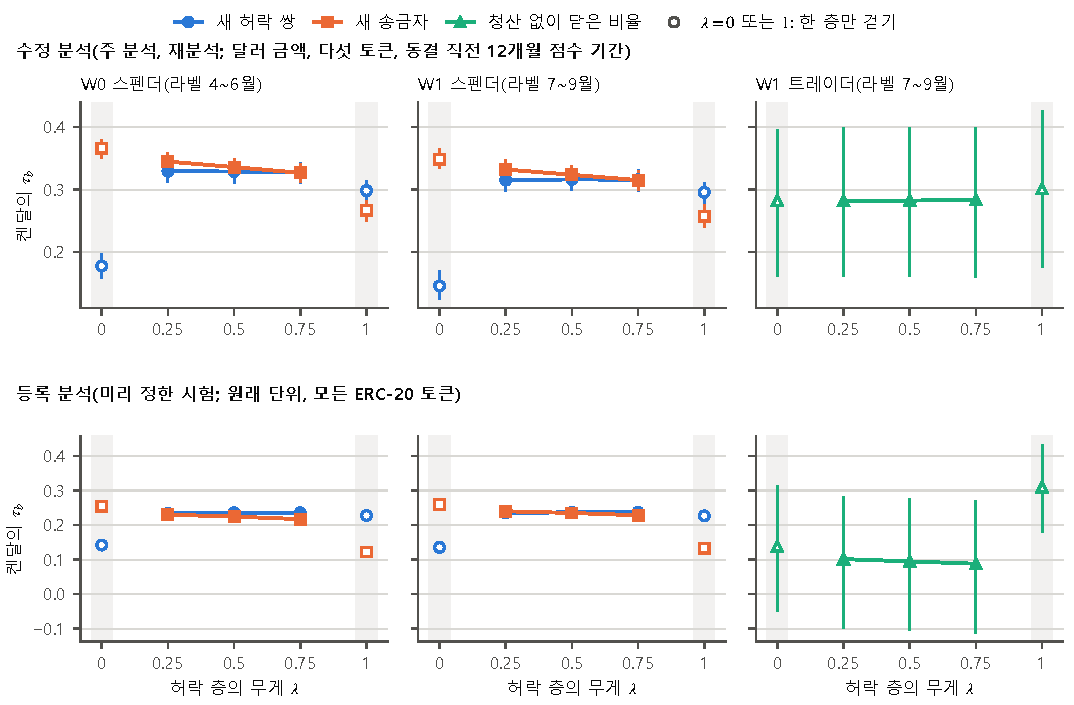
\includegraphics[width=\linewidth]{figures/fig_lambda_sweep.pdf}
\caption{허락 층의 무게 $\lambda$에 따른, C-PR과 각 나중 라벨 사이의 켄달 $\tau_b$와 95\% 짝지은 부트스트랩 구간. 선으로 이은 채운 표시는 미리 정한 격자 $\lambda\in\{0.25,0.5,0.75\}$예요. 회색 띠 안의 빈 표시는 $\lambda=0$과 $\lambda=1$, 곧 송금 걷기와 허락 걷기예요. 선이 잇지 않는 별개의 연산자예요. 위 줄은 수정 분석(주 분석, 재분석), 아래 줄은 등록 분석(미리 정한 시험)이에요. 줄마다 세로축을 같이 써요. 값은 표~\ref{tab:holdout}에 있어요.}
\label{fig:sweep}
\end{figure}

\subsection{씨앗 재시작}

S-PR은 새 송금자에서는 송금 걷기에 가깝고, 새 허락 쌍에서는 허락 걷기보다 한참 아래에 머물러요.
\begin{itemize}
\item W0에서 새 허락 쌍의 S-PR − 허락 걷기는 수정 분석에서 −0.108 [−0.128, −0.088], 등록 분석에서 −0.051 [−0.060, −0.043]이에요.
\item 새 송금자의 S-PR − 송금 걷기는 +0.011 [0.004, 0.018]과 −0.009 [−0.012, −0.006]이에요.
\item 다시 출발은 새 허락 쌍의 계수를 송금 걷기에서 허락 걷기 쪽으로 일부만 끌어올려요. 수정 W0에서 0.190이고 송금 걷기는 0.178, 허락 걷기는 0.298이에요. 등록 W0에서는 0.177 대 0.142와 0.228이에요. 송금 걷기와의 짝지은 대비는 계산하지 않았어요.
\end{itemize}
$d=0.85$이면 몫의 15\%와 매달린 점의 몫만 다시 출발 벡터를 지나요. 그래서 허락 화살표는 걷기를 실어 나를 때, 곧 허락 걷기에서는 온전히, C-PR에서는 섞여서 쓰일 때 나중 허락에 도움이 되고, 다시 출발할 곳만 정할 때는 거의 도움이 되지 않아요.

나중 송금자에서는 순서가 뒤집혀요. 라벨을 안 뒤에 수정 점수 파일로 계산한 대비에서, C-PR은 두 창 모두에서 새 허락 쌍은 S-PR보다 더 잘 줄 세우지만(+0.139 [0.121, 0.156], +0.154 [0.134, 0.174]), 새 송금자는 S-PR만큼 잘 줄 세우지 못해요(−0.041 [−0.049, −0.032], −0.044 [−0.052, −0.037]).

\subsection{걷기 대 수}

어떤 걷기도 새 허락 쌍을 원시 받은 허락 수만큼 잘 줄 세우지 못했어요. 두 분석 모두 점 추정값으로 그랬고, 계산한 짝지은 대비마다 그랬어요.
\begin{itemize}
\item \textbf{W0.} 허락 걷기는 받은 허락 수에 수정 분석에서 −0.094 [−0.104, −0.083], 등록 분석에서 −0.025 [−0.030, −0.019]만큼 모자라요. 엔도스랭크는 −0.090 [−0.100, −0.079]와 −0.011 [−0.016, −0.006]만큼 모자라요.
\item \textbf{W1.} 엔도스랭크는 −0.082 [−0.090, −0.073]과 −0.029 [−0.032, −0.025]만큼 모자라요. 허락 걷기의 점 추정값도 받은 허락 수보다 낮아요(0.295 대 0.381, 0.227 대 0.262). 짝지은 대비는 계산하지 않았어요.
\item \textbf{라벨을 안 뒤에 수정 점수 파일로 계산한 짝지은 대비.} C-PR은 두 창 모두에서 받은 허락 수에 모자라요(−0.063 [−0.076, −0.052], −0.065 [−0.077, −0.054]). AWP의 활동 재시작을 쓴 엔도스랭크도 그래요(−0.060 [−0.070, −0.052], −0.046 [−0.055, −0.038]). 등록 분석에서 C-PR의 새 허락 쌍 점 추정값은 두 창 모두 받은 허락 수보다 아래예요(표~\ref{tab:holdout}). 짝지은 대비는 계산하지 않았어요.
\end{itemize}

새 송금자에서도 수정 분석에서는 수가 앞서요. C-PR은 두 창 모두에서 새 송금자를 송금 입차수만큼 잘 줄 세우지 못하고(−0.111 [−0.121, −0.100], −0.115 [−0.128, −0.105]), AWP도 그래요(W0 −0.038 [−0.043, −0.032], W1 −0.041 [−0.047, −0.034]). 반면 등록 분석에서는 AWP가 송금 입차수보다 더 잘 줄 세워요(+0.038 [0.035, 0.042], +0.020 [0.016, 0.023]). 균등 재시작과 상한 없는 금액을 쓰는 C-PR의 송금 걷기는, 모든 경우에 송금 입차수보다 점 추정값이 낮아요.

기준 비교는 짝 연구가 모두 보고해요~\cite{kwon2026companion}. 여기서 되풀이하는 까닭은, 이 비교가 이 원고의 어떤 걷기든 주장할 수 있는 범위를 묶기 때문이에요. 허락 쪽은 명제~\ref{prop:closed}가 설명해요. 대부분의 스펜더에서 걷기는 무게를 다시 단 주인 수이고, 이 도착 라벨에서는 다시 단 무게가 도움이 되지 않았어요. 차수 결과는 선호적 연결~\cite{barabasi1999scaling,newman2001clustering}, 그리고 링크 예측에서 차수 기준선이 강하다는 것~\cite{libennowell2007link,lin2022tracking}과 맞아요.

\subsection{라벨을 본 뒤, 기준 걷기와 견주기}
\label{sec:reference}

규칙 A와 B는 C-PR을 자기 층과 견줘요. 결합만을 바꾸는 대비는 그것뿐이기 때문이에요. 짝 연구의 기준 걷기와의 대비는 라벨을 안 뒤에 수정 점수 파일로, 규칙과 같은 다시 뽑기를 써서 계산했어요. 이 대비들이 C-PR의 자리를 더 밝혀 줘요. 어느 것도 규칙에 들어가지 않고, 표~\ref{tab:contrasts}의 두 행 말고는 등록 분석에 짝이 없어요.
\begin{itemize}
\item \textbf{엔도스랭크와.} 각 스펜더 라벨과 각 창에서 C-PR이 앞서요. 새 허락 쌍에서 +0.026 [0.016, 0.037]과 +0.017 [0.006, 0.029], 새 송금자에서 +0.064 [0.052, 0.075]와 +0.064 [0.051, 0.076]이에요.
\item \textbf{활동 재시작 엔도스랭크와.} 새 허락 쌍에서 W0에서는 같고(−0.003 [−0.014, 0.008]), W1에서는 못해요(−0.019 [−0.029, −0.008]).
\item \textbf{AWP와.} 새 허락 쌍에서 C-PR이 앞서는 것(W0 +0.133 [0.114, 0.153], W1 +0.159 [0.139, 0.178], S1의 F1)은 대부분 송금 화살표가 없어서 AWP가 0점을 주는 스펜더에서 와요. 동결 전에 들어온 송금이 있는 스펜더(W0 6,489개, W1 6,567개)만 보면, 새 허락 쌍에서 C-PR과 AWP는 W0에서 같고(+0.008 [−0.002, 0.020]) W1에서 C-PR이 0.022 [0.011, 0.033] 앞서요. 반면 새 송금자에서는 AWP가 0.036 [0.026, 0.044]와 0.037 [0.028, 0.046]만큼 더 잘 줄 세워요. 모든 스펜더에서도 그랬어요(W0에서 0.073 [0.063, 0.083], W1에서 0.075 [0.065, 0.085]).
\end{itemize}
그러니 기간 밖에서 허락 층이 송금 걷기에 더해 주는 것은 주로, 송금 걷기가 동점으로 남겨 두는 계약들 사이의 순서예요. 나머지 계약들 사이에서는 W1에서 나중 허락에 작은 앞섬이 있을 뿐이에요. 나중 송금자에서는 C-PR이 모든 부분 집합과 창에서 AWP보다 뒤져요.

\subsection{정밀도와 허용 폭}
\label{sec:precision}

허용 폭은 스펜더 대비의 정밀도에서 나왔고, 그대로 트레이더 대비에 적용했어요.
\begin{itemize}
\item \textbf{스펜더에서는 지킬 수 있는 폭이었어요.} F2의 구간 폭은 수정 분석에서 0.023, 등록 분석에서 0.008이에요. F2가 실패한 것은 구간이 넓어서가 아니라, 구간 전체가 허용 폭 너머에 있었기 때문이에요.
\item \textbf{트레이더에서는 계약 70개로 겨우 닿는 폭이었어요.} F3의 구간 폭은 수정 분석에서 0.020, 등록 분석에서 0.098이에요. 두 계수가 같으면, 수정 F3은 구간이 약 $2\delta$보다 좁을 때만 성립할 수 있어요. 등록한 시드에서 반폭은 0.01004이고, 다른 부트스트랩 시드 50개에서 아래 끝은 −0.0146에서 −0.0098 사이이며, 한 시드에서는 아래 끝이 −0.01보다 위로 올라와 기준을 통과해요(부록~\ref{app:explore}).
\end{itemize}
그래서 수정 F3의 실패는 두 걷기의 차이가 아니라 다시 뽑기에 달려 있어요. 반면 등록 분석의 반폭(0.049)은 허용 폭의 약 5배이고, 등록 F3의 위 끝은 시드 50개 가운데 11개에서 0 이상에 닿아요. 스펜더 구간의 끝은 시드에 따라 거의 움직이지 않고(표준편차 0.0002–0.0015), 규칙 B는 F2 때문에 두 분석의 모든 시드에서 실패해요.

스펜더 쪽 라벨은 듬성듬성해요. 수정 W1 스펜더 7,960개 가운데 1,495개만 새 허락 쌍을, 1,371개만 새 송금자를 얻었어요(등록 분석에서는 34,587개 가운데 2,850개와 2,812개). 그래서 스펜더 계수는 저마다 그 부분 집합들의 순서에 크게 기대요.

\begin{puri}[허용 폭을 지키려면 구간이 얼마나 좁아야 하나요?]
두 계수가 같으면 차이의 점 추정값이 0이에요. 비열등성은 아래 끝이 −0.01보다 위에 있어야 하므로, 구간의 아래쪽 반이 0.01보다 짧아야 해요. 곧 구간 전체의 폭이 약 $2\delta$보다 좁아야 해요. 수정 F3의 폭은 0.020이라 딱 그 경계에 걸렸고, 시드에 따라 통과하기도 해요. 등록 F3은 반폭이 0.049라, 계수가 같았더라도 통과할 수 없는 폭이었어요.
\end{puri}
